\chapter{Tecnologías y Herramientas} 
\label{sec:tecnologia}

\section{Postman}

Es una herramienta muy útil, orientada a los desarrolladores, que permite realizar peticiones de una forma sencilla e intuitiva a cualquier API. En este proyecto se ha usado Postman para comprobar el correcto funcionamiento de la API desarrollada.

\section{Git}

Es un programa para el control de versiones que permite: mantener un historial de todos los cambios realizados en el código de un proyecto y coordinar el trabajo de un equipo sobre archivos compartidos.
En este proyecto se ha utilizado Git para subir los cambios a un repositorio externo; sin embargo, no se han tenido que utilizar distintas ramas de desarrollo porque todo el trabajo ha sido individual.

\section{Github}

Es un sitio web destinado al alojamiento de código que utiliza Git. Se caracteriza por sus funciones colaborativas permitiendo que cualquier persona pueda visualizar y descargar el código fuente, sugerir cambios y ayudar a mejorar el proyecto. Si un usuario desea restringir el acceso a su repositorio pueden crearse proyectos privados.

\section{Trello}

Es una herramienta creada para facilitar la gestión de proyectos, que cuenta con una interfaz web y un cliente para iOS y Android. Permite crear y organizar tareas en forma de "tarjetas" y organizarlas en diferentes bloques. Cada uno de estos bloques se identifica con una etapa diferente del flujo de trabajo, de modo que durante el desarrollo las tarjetas se van moviendo de un bloque a otro para identificar el estado actual de la tarea. 


\section{Visual Studio Code}

Se encuentra a medio camino entre un editor de texto y un IDE. Fue desarrollado por Microsoft y es multiplataforma (Windows, Linux y macOS). Gracias al amplio ecosistema de plugins que posee permite trabajar con una gran cantidad de lenguajes de programación (Go, Python, C, C++, etc.). Incluye funcionalidades como la finalización de código inteligente, refactorización de código, soporte de depuración, entre otros.

\section{Xampp}

Es la herramienta más utilizada para la instalación de entornos de desarrollo, consistente en un conjunto de herramientas que se enumeran a continuación:

\begin{itemize}
    \item \textbf{MariaDB}. Es un sistema de gestión de bases de datos creado a partir de MySQL. MariaDB nació como una bifurcación directa de MySQL cuando éste fue adquirido por Oracle para asegurar que se mantuviese como software libre. MariaDB cuenta con todas las funcionalidades de MySQL, aunque añade otras relacionadas con los mecanismos de almacenamiento y la facilidad de uso.  
    \item \textbf{Apache}. Es un servidor web HTTP de código abierto y multiplataforma que destaca por su facilidad de uso y popularidad. Apache implementa el protocolo HTTP/1.1.
    \item \textbf{Perl}. Se trata de un lenguaje de programación inspirado en lenguajes como C, Shell y AWK, entre algunos otros. Fue ampliamente adoptado por su facilidad para el procesamiento de textos, tareas como extraer información y generar informes a partir del contenido de archivos de texto.
    \item \textbf{PHP}. Es el lenguaje más utilizado para el desarrollo web en el lado del servidor. En un principio era conocido como Personal Home Page Tools y se trataba de un CGI capaz de interpretar unos pocos comandos. Durante el paso de los años fue objeto de una serie de mejoras que lo han convertido en lo que hoy conocemos por PHP (PHP: Hypertext Preprocessor).
\end{itemize}

\section{Wordpress}
En primer lugar, es necesario definir el concepto de CMS (Content Management System). Como su propio nombre indica, se trata de una aplicación software o un conjunto de programas relacionados que son usados para la creación y administración de contenido digital. 

Alrededor de un 60\% de las páginas web que podemos encontrar hoy en día hacen uso de un CMS. De entre todas esas páginas, el 64,3\% están construidas con Wordpress \citeW{W3Techs:1}. En la siguiente figura se puede observar la tendencia de uso que han seguido los diferentes CMS a lo largo de los últimos diez años \citeW{W3Techs:2}: 

\begin{figure}[ht]
	\begin{center}
		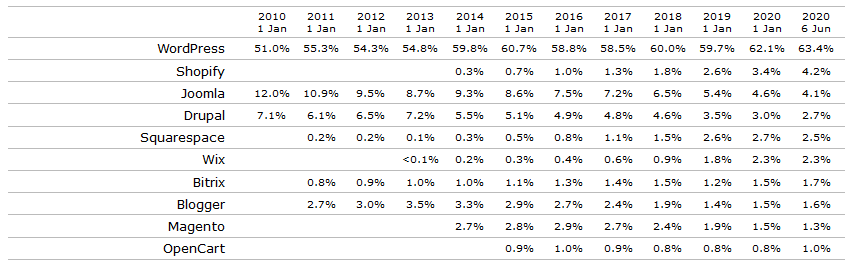
\includegraphics[width = 0.95\textwidth]{Figuras/TendenciaUsoCMS.PNG}
	\end{center}
	\caption{\label{fig:CMS} Tendencia de uso de los CMS. Fuente: W3Techs.}
\end{figure}

Como se puede observar, Wordpress ha sido el líder de los CMS durante diez años seguidos y presenta una diferencia muy notable respecto a su competidor más cercano.

Por ser el más popular cuenta con una gran variedad de plantillas de diseño y plugins que permiten añadir cualquier tipo de funcionalidad que se pueda imaginar. Haciendo uso de uno estos plugins, se puede implementar una tienda virtual de forma sencilla e intuitiva sin requerir de conocimientos técnicos avanzados. Es por esta razón por la que gran parte de las pymes diseñan sus sitios webs utilizando Wordpress.

Al adoptar esta tecnología se pretende demostrar que cualquier empresa dedicada al comercio electrónico puede incorporar herramientas de IA en su tienda en línea.

\newpage

\subsection{WooCommerce}

Se trata de una extensión gratuita para Wordpress que permite transformar una página web en una tienda de comercio electrónico en cuestión de minutos. Aunque la venta de productos es el escenario más obvio para la creación de una tienda, WooCommerce también soporta la creación de webs destinadas a la venta de servicios o suscripciones. 
Es la plataforma de comercio electrónico líder en 2020 con un 28,24\% de cuota de mercado \citeW{statista}:

\begin{figure}[ht]
	\begin{center}
		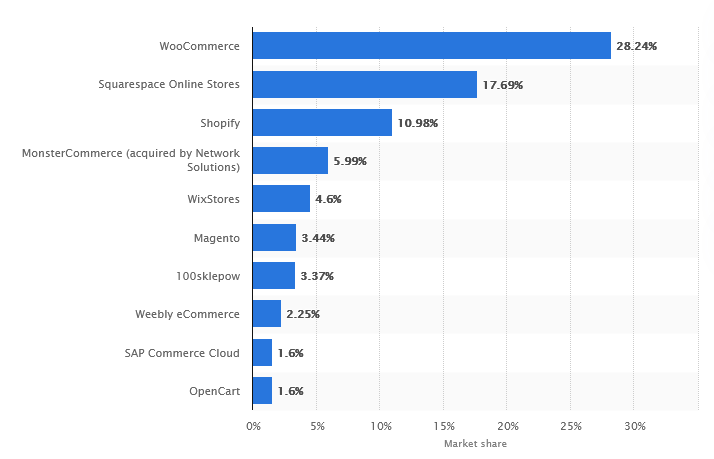
\includegraphics[width = 0.80\textwidth]{Figuras/eCommerceMarketShare.PNG}
	\end{center}
	\caption{\label{fig:WooCommerce} Cuota de mercado de las principales plataformas de comercio electrónico. Fuente: Statista.}
\end{figure}

Existen más de 50.000 plugins de Wordpress específicamente desarrollados para WooCommerce, ofreciendo al usuario la capacidad de personalizar completamente su tienda.

\subsection{MyChatbot}

De manera sencilla, se puede definir un chatbot como un servicio de software que responde automáticamente a las preguntas que se le plantean a través de una interfaz de chat. Su uso en el comercio electrónico permite aportar soluciones a los clientes las 24 horas del día sin necesidad de que participe ningún empleado.

Existen multitud de plugins que permiten incorporar un bot conversacional a Wordpress,  la mayoría de éstos ofrecen un sistema entrenado o cuentan con un constructor para facilitar la tarea a los usuarios. Sin embargo, en este trabajo sólo se pretende conectar Wordpress con un motor conversacional desarrollado en una plataforma externa.

Con este objetivo se ha elegido MyChatbot, una herramienta gratuita que utiliza Dialogflow —plataforma de comprensión del lenguaje natural perteneciente a Google— como motor conversacional. Seguidamente se muestra un ejemplo de este plugin:

\begin{figure}[ht]
    \begin{center}
    	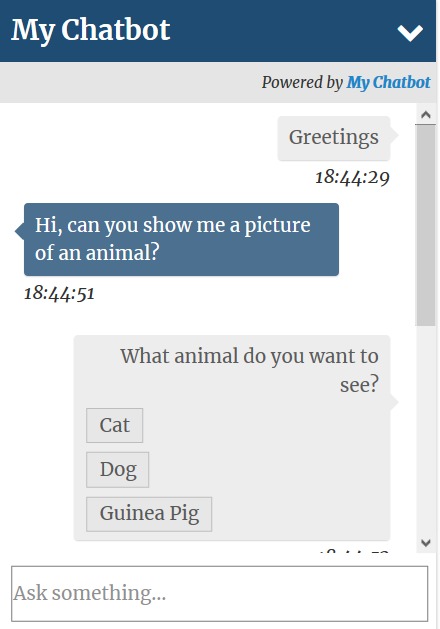
\includegraphics[width = 0.30\textwidth]{Figuras/chatbotExample.PNG}
    \end{center}
    \caption{\label{fig:myChatbot} Ejemplo de MyChatbot en funcionamiento. Fuente: My Chatbot WordPress plugin demo.}
\end{figure}

\subsection{WP-Stateless}
La página web implementada será desplegada haciendo uso de Cloud Run. Esta plataforma ejecuta contenedores sin estado, por tanto, los cambios que se realicen durante la ejecución del contenedor no se guardarán si se reinicia el servicio. No obstante, esta característica no tiene impacto sobre aquella información que se almacena en la base de datos, pero sí afecta a los archivos multimedia, como las imágenes que ilustran un producto.

WP-Stateless es una extensión de Wordpress que almacena todos los archivos que se suben en un segmento de Google Cloud Storage para hacerlos persistentes. En cuanto a su configuración, el proceso es muy sencillo, tan sólo se debe elegir un proyecto existente de Google Cloud y el resto de campos se completará automáticamente.

\newpage

\section{GoLang}

Go es un lenguaje de programación multiplataforma moderno, muy potente y simple. Es una elección excelente para aplicaciones cloud y orientadas a microservicios. Go está ganando popularidad a pasos agigantados y está atrayendo a muchos programadores. Tal es el hecho, que en la encuesta realizada por StackOverflow a 65000 desarrolladores, Go figura como el quinto lenguaje favorito y el tercero más buscado \citeW{StackOverflow}. A continuación, se muestran los resultados de dicha encuesta: 

\begin{figure}[ht]
	\begin{center}
		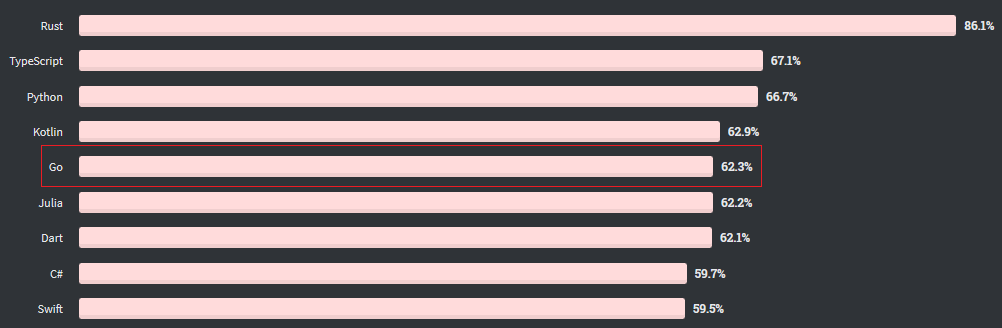
\includegraphics[width = 0.95\textwidth]{Figuras/queridos.png}
	\end{center}
	\caption{\label{fig:Loved} Lenguajes favoritos de los desarrolladores en 2020. Fuente: StackOverflow.}
\end{figure}

\begin{figure}[ht]
	\begin{center}
		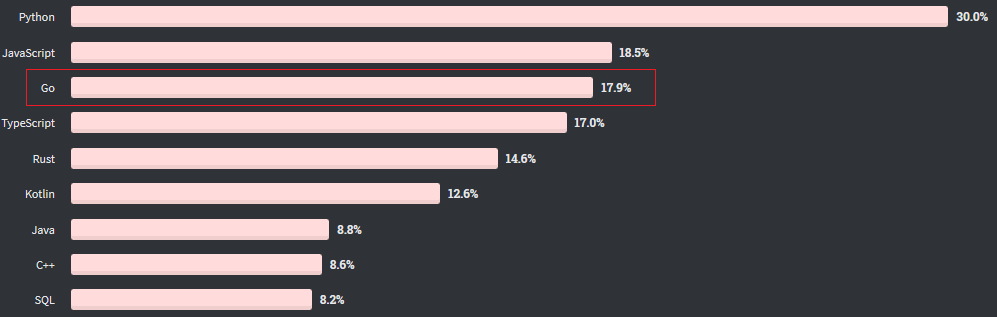
\includegraphics[width = 0.95\textwidth]{Figuras/buscados.png}
	\end{center}
	\caption{\label{fig:Wanted} Lenguajes más buscados por los desarrolladores en 2020. Fuente: StackOverflow.}
\end{figure}

\section{Dockers}

Un contenedor es una unidad de software que empaqueta el código y todas sus dependencias para que la aplicación pueda ejecutarse en cualquier entorno informático asegurando su funcionamiento uniformemente a pesar de las diferencias como, por ejemplo, desarrollo y producción. Una imagen de contenedor es un paquete de software ligero, independiente y ejecutable que incluye todo lo necesario para ejecutar una aplicación: código, herramientas del sistema, librerías y configuraciones.

En el caso de los contenedores Docker, su imagen se convierte en contenedor al ejecutarlo con Docker Engine \citeW{Docker}. 

A menudo, las personas que se inician en esta tecnología tienden a confundirla con la funcionalidad de los contenedores tradicionales de Linux. Si bien es verdad que Docker surgió a partir de la tecnología LXC (Linux containers), actualmente se encuentra muy alejado de su influencia. LXC sólo era un método de virtualización ligera. Sin embargo, Docker va más allá, no sólo provee la capacidad de crear contenedores sino que también ofrece un flujo de trabajo, ayudando a la creación y diseño de contenedores y al envío y creación de versiones de imágenes \citeW{RedHat}.

La tecnología Docker tiene un enfoque granular, en el sentido de que pretende conseguir la separación de las aplicaciones en sus procesos individuales y además ofrece las herramientas para ello. En la siguiente figura se realiza una comparación de ambas tecnologías:

\begin{figure}[ht]
	\begin{center}
		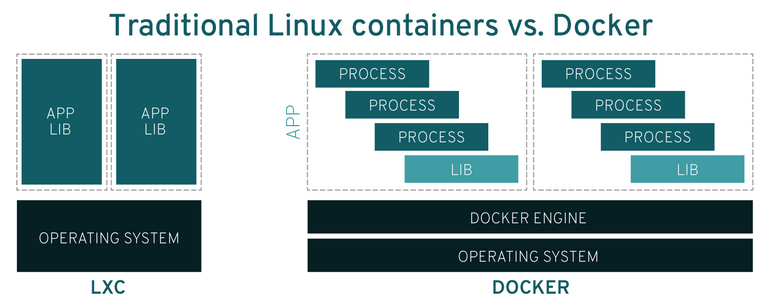
\includegraphics[width = 0.95\textwidth]{Figuras/Docker_LXC.PNG}
	\end{center}
	\caption{\label{fig:Docker_LXC} Comparación de LXC y Docker. Fuente: Red Hat.}
\end{figure}

Docker-Engine esta formado por tres componentes principales:
\begin{itemize}[leftmargin=+.5in]
    \item Un cliente (\textit{docker}), por medio del cual se pueden ejecutar diferentes comandos como \textit{build}, \textit{run}, \textit{rm}, \textit{push}, \textit{pull}, etc. 
    \item Un servidor (\textit{dockerd}), al que también se puede hacer referencia como demonio si se tiene en cuenta la notación de linux.
    \item Una API REST (\textit{docker registry}), que especifica las interfaces que los programas pueden usar para hablar con el servidor o demonio e indicarle qué hacer.
\end{itemize}

\newpage

A continuación, se presenta en una figura los componentes Docker Engine:

\begin{figure}[ht]
	\begin{center}
		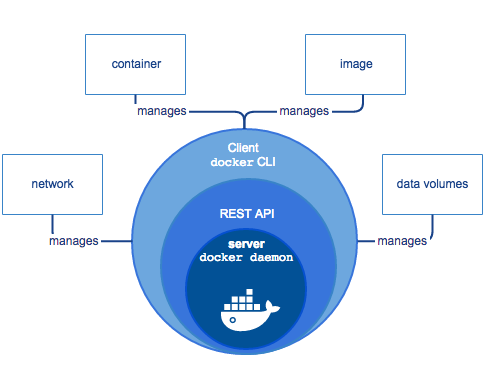
\includegraphics[width = 0.60\textwidth]{Figuras/DockerComponents.png}
	\end{center}
	\caption{\label{fig:DockerComponents} Componentes de Docker Engine. Fuente: docker docs.}
\end{figure}

El cliente Docker interactúa con el demonio Docker, que hace el trabajo pesado de construir, ejecutar y distribuir sus contenedores. El cliente y el demonio pueden ejecutarse en el mismo sistema, o se puede realizar una conexión con un cliente o demonio remotos. Ambos se comunican mediante una API REST, a través de sockets UNIX o una interfaz de red.

\begin{figure}[ht]
	\begin{center}
		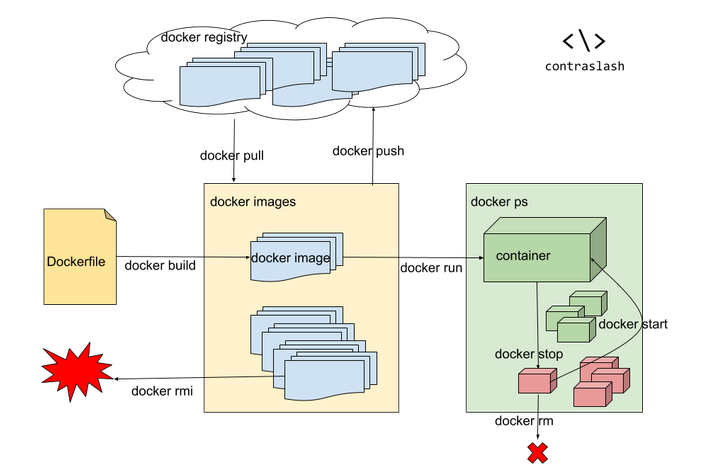
\includegraphics[width = 0.80\textwidth]{Figuras/DockerArchitecture.png}
	\end{center}
	\caption{\label{fig:DockerArchitecture} Arquitectura de Docker. Fuente: contraslash.}
\end{figure}

\section{Servicios cloud de Google}

Para la realización del proyecto se han utilizado diferentes servicios disponibles en Google Cloud. ¿Por qué? Uno de los objetivos del trabajo es desplegar la página web y la aplicación en la nube mediante contenedores. Existen muchas plataformas para realizar este proceso y cada una cuenta con herramientas específicas para ello. Mientras se investigaba sobre todas estas posibilidades, surgió la de utilizar Cloud Run, una plataforma de computación en la nube sin servidores y que fue lanzada al mercado por Google hace tan sólo un año. Este servicio encaja con las necesidades del proyecto, al mismo tiempo que supone un reto, ya que, al ser tan reciente, en la web no se pueden encontrar tantos ejemplos de su uso como de otras opciones. Asimismo, entre los servicios de procesamiento del lenguaje natural, se determinó que uno de los más adecuados era el de Google, debido a que devuelve un valor decimal comprendido entre -1 y 1 que puede ser discretizado para su representación en forma de estrellas. Al optar por dos herramientas de Google Cloud se decidió utilizar esta plataforma para el resto de funcionalidades necesarias.

En esta sección se expondrán cuáles son estos servicios, su rol y la razón de su elección.

\subsection{Google Natural Language Processing}

Esta herramienta permite el análisis de opiniones, el análisis de entidades, el análisis de opiniones sobre entidades, la clasificación de contenido y el análisis sintáctico. El análisis de un texto mediante esta herramienta da como resultado dos valores numéricos:

\begin{itemize}
    \item \textbf{Puntuación}. Número decimal comprendido entre -1,0 (negativo) y 1,0 (positivo). Se corresponde con la tendencia emocional general del texto.
    \item \textbf{Magnitud}. Número decimal comprendido entre 1,0 e $\infty$. Expresa la intensidad de la emoción. Hay que tener en cuenta que para el cálculo de este valor se considera cada expresión de emoción en el texto. Por tanto, los valores de magnitud para textos más largos es probable que sean mayores.
\end{itemize}

Es importante resaltar que este servicio sólo diferencia entre emociones positivas o negativas, pero no es capaz de identificar emociones específicas (furia, sorpresa, tristeza, etc.). 

Para ilustrar el modo de funcionamiento, se procede a analizar la siguiente opinión de un usuario sobre el libro \textit{El lobo estepario} de Herman Hesse en Amazon: “A good read. Smart. But moody and not too readable. But I still remember the story, so it has influence on you.”

\newpage

La salida obtenida al hacer una petición a Google NLP es:

\begin{lstlisting}[caption=Ejemplo de respuesta API NLP ]
"documentSentiment": {
    "magnitude": 2.0,
    "score": 0.4
  },
language": "en",
  "sentences": [
    {...}
  ]
}
\end{lstlisting}

Ofrece una puntuación de 0,4  y magnitud de 2,0 para la opinión de forma general y continúa desgranando los valores para cada una de las frases que la forman. Se puede observar que existe una fuerte intensidad de la emoción, debido a que se alcanza un valor de 2 en un texto formado por dos líneas. A su vez, la puntuación indica que se trata de una opinión positiva, aunque no demasiado.

Si la opinión tiene una puntuación cercana a cero puede deberse a que la intensidad de la emoción es baja o a que presenta emociones mixtas. Por ello, antes de clasificar dicha opinión es necesario eliminar la ambigüedad atendiendo a la magnitud, ya que las opiniones que sean verdaderamente neutrales tendrán un valor de magnitud bajo, mientras que las opiniones con emociones mixtas tendrán un valor alto.

Este servicio presenta una ventaja frente a sus principales competidores porque además de ofrecer una puntuación que oscila en un intervalo, también permite eliminar ambigüedades con otro parámetro de la respuesta.

\subsection{Cloud Run}

Realizar el despliegue de una página web puede llegar a convertirse en una tarea tediosa si se tiene en cuenta la sobrecarga de trabajo que conlleva la creación y administración de clústers, servicios, grupos de contenedores, máquinas virtuales, etc. Esta situación es aceptable si se está tratando con grandes aplicaciones formadas por varios niveles, pero si sólo se desea desplegar y hacer visible un sitio web, es una carga demasiado grande.

Cloud Run permite administrar y desplegar una página web haciendo que el usuario se desentienda de cualquier aspecto relacionado con de la infraestructura y disponibilidad. Se trata de una plataforma que ejecuta contenedores sin estado, esto quiere decir que cualquier cambio que se introduzca en la página web o aplicación durante su ejecución no será persistente. Para afrontar esta situación se pueden tomar dos decisiones, realizar los cambios en local y subir nuevas revisiones o añadir volúmenes al contenedor. 

Cada implementación de un nuevo servicio en Cloud Run crea una revisión. Dicha revisión está compuesta por una imagen de contenedor, la configuración del entorno, las variables de entorno, los límites de memoria y el valor de simultaneidad. Las revisiones son inmutables, es decir, una vez creadas no se podrán modificar. Si se añade una nueva imagen a ese mismo servicio, se crea una nueva revisión. Cuando se modifican los límites de memoria, se crea otra nueva revisión, etc.

Las revisiones que se encuentren recibiendo peticiones escalan automáticamente a la cantidad de contenedores necesarios para hacerse cargo de todas las solicitudes. Además, cuando la revisión no esté recibiendo ninguna petición escalará el número de contenedores a cero. La cantidad máxima de solicitudes que se pueden enviar en paralelo a una instancia de contenedor se puede configurar mediante el valor de simultaneidad \citeW{CloudRun}. 

\subsection{Cloud SQL}
Para su funcionamiento, Wordpress necesita una base de datos MySQL donde almacenar toda la información de la página web, la configuración de los plugins y de los temas.

CloudSQL es un servicio de bases de datos totalmente administrado que es compatible con MySQL, PostgreSQL y SQL Server. En general, las funciones de MySQL que proporciona una instancia de Cloud SQL son las mismas que las que proporciona una instancia de MySQL alojada localmente \citeW{CloudSQL}. 

A la hora de crear la instancia se ofrecen distintas opciones de configuración al usuario:

\begin{itemize}
    \item \textbf{Tipo de almacenamiento}
    \begin{itemize}
        \item SSD. Ofrece un número de consultas por segundo y rendimiento de datos más altos.
        \item HDD. Tiene un rendimiento más bajo comparado con el SSD. Esta opción es la más económica.
    \end{itemize}
    \item \textbf{Capacidad de almacenamiento}
    \newline
    El rendimiento y la capacidad de la instancia son proporcionales. También se puede activar la opción "Habilitar los aumentos automáticos de almacenamiento" permitiendo así que el espacio de almacenamiento aumente cada vez que se esté cerca de alcanzar la capacidad establecida.
    \item \textbf{Copias de seguridad}
    \newline
    Realizar de forma automática las copias de seguridad en el horario seleccionado.
    \item \textbf{Disponibilidad}
     \begin{itemize}
        \item Zona única. En caso de que se produzca una interrupción no se activa la conmutación por error. Esta opción es poco recomendable para instancias de producción.
        \item Alta disponibilidad(regional). Activa la conmutación por error automática hacia otra zona dentro de la región que ha sido seleccionada. Esta opción es más costosa.
    \end{itemize}
    \item \textbf{Mantenimiento}
    \newline
    Permite seleccionar el período de tiempo para llevar a cabo este proceso, ya que durante el mantenimiento la instancia se reinicia, de modo que el servicio se ve interrumpido brevemente.
\end{itemize}

Para la realización de este proyecto se ha hecho uso de una instancia de tipo \textit{db-f1-micro}, que es la configuración más básica permitida y sólo está recomendada para entornos de desarrollo y prueba.

\subsection{Container Registry}

Se trata de un registro privado de imágenes de contenedor que se ejecuta en Google Cloud. Será aquí donde se almacenen las imágenes de contenedor utilizadas en el proyecto. 

Dentro del registro se pueden almacenar multitud de imágenes y cada una de ellas puede constar de varias versiones. Es posible identificar una versión específica de una imagen dentro de un registro haciendo uso de etiquetas (exclusivas a nivel de registro) \citeW{Registry}. 

Cloud Run puede extraer imágenes de Container Registry para ejecutar un servicio y, aunque no sea este el caso, Container Registry también puede integrarse con servicios externos, como por ejemplo, Kubernetes.

\subsection{Cloud Logging}

Es una herramienta de Google Cloud que permite almacenar, buscar, analizar y monitorizar eventos y datos de registros, así como crear registros personalizados haciendo uso de su API. Cuenta con un visor que permite seleccionar entradas de registro filtrando por diferentes opciones, como un periodo específico, nivel de gravedad, origen, etc. En la siguiente figura se muestra el aspecto del visor de registros:

\begin{figure}[ht]
	\begin{center}
		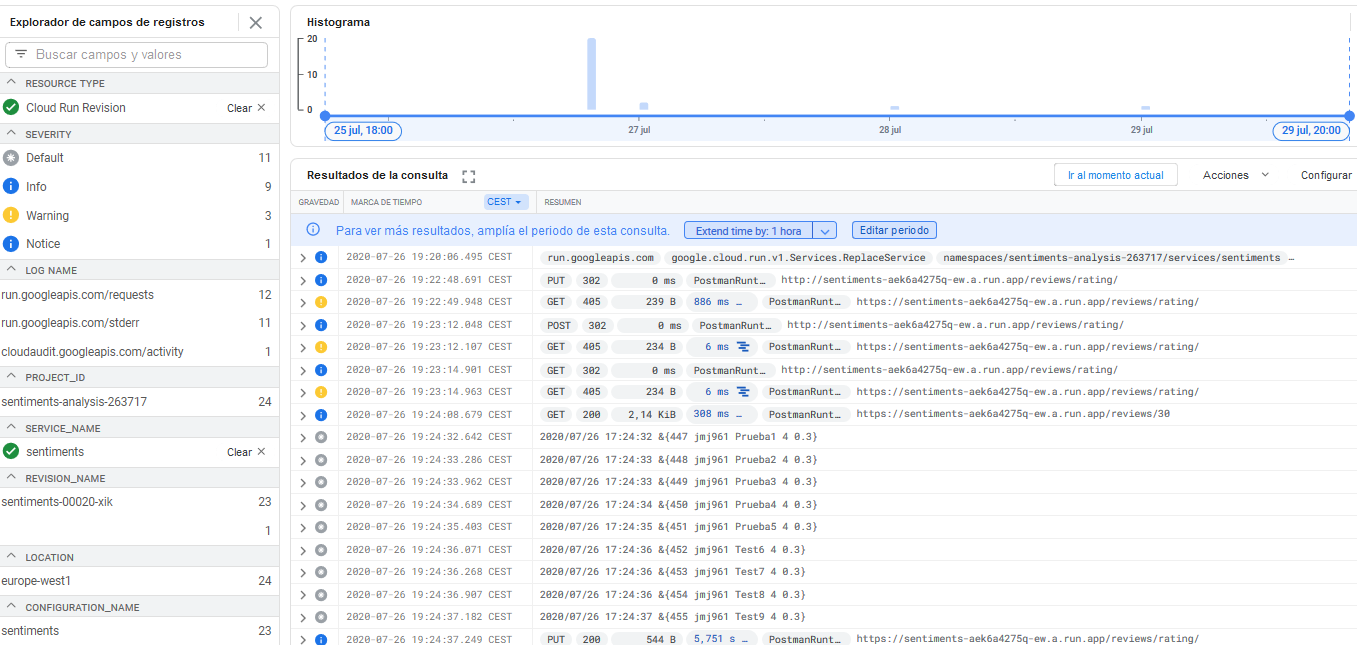
\includegraphics[width = 1\textwidth]{Figuras/cloudLogging.PNG}
	\end{center}
	\caption{\label{fig:cloudLogging} Visor de registros Cloud Logging}
\end{figure}

\newpage

Gracias a esta herramienta es posible gestionar y analizar los registros personalizados que se incluyen en la aplicación de análisis de sentimientos con el objetivo de identificar y solucionar rápidamente el origen de los posibles problemas que surjan.

\subsection{DialogFlow}

Se trata de una herramienta de Google Cloud que permite crear modelos que sean capaces de interpretar las intenciones del usuario y extraer información relevante de las conversaciones, todo ello a través de una interfaz de usuario visual que no requiere de experiencia en aprendizaje automático \citeW{DialogFlow}. 

\begin{figure}[ht]
     \begin{center}
        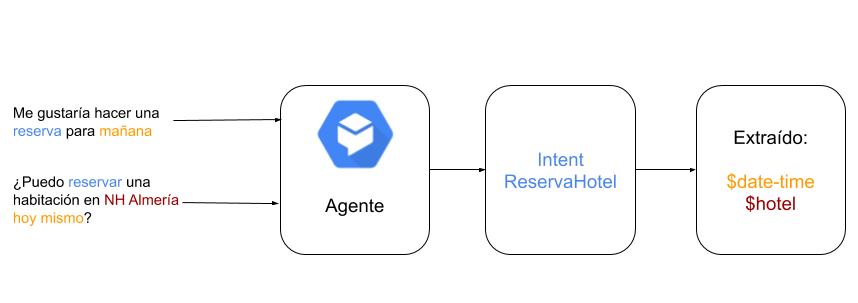
\includegraphics[width = 0.90\textwidth]{Figuras/IntentsDiagram.png}
     \end{center}
     \caption{\label{fig:IntentsDiagram}Diagrama de funcionamiento}
\end{figure}

\newpage

Para comprender su funcionamiento es necesario conocer los conceptos de:
\begin{itemize}
     \item \textbf{Agentes}. Se debe ver a un agente de DialogFlow como si se tratase, por ejemplo, de un trabajador en un centro de llamadas. Al igual que el empleado en sus primeros días de trabajo, el agente debe ser entrenado para manejar las conversaciones con los clientes. 
     
     DialogFlow traduce la entrada de texto que recibe por parte del usuario durante la conversación a datos estructurados que puedan ser utilizados por una aplicación o servicio.
    
     \item \textbf{Intents}. Básicamente es cómo determina DialogFlow lo que un usuario desea hacer. Permiten definir un conjunto de tareas individuales que pueden ser invocadas por el usuario. Es conveniente crear intents cuya funcionalidad esté centrada en el propósito de su creación, para que la duración de la invocación sea breve, ofreciendo así al usuario la respuesta adecuada en un intervalo de tiempo más corto.
     
     Un intent está formado por los siguientes elementos:
     \begin{itemize}
         \item Frases de entrenamiento. Son frases que el usuario puede decir para activar el intent. No es necesario definir todas las variantes posibles de una frase, ya que el aprendizaje automático que está integrado en la herramienta extiende la lista definida con otras frases parecidas.
         \item Acción. Cuando Dialogflow identifica una coincidencia con un intent, transmite la acción al sistema que puede ser usada para activar otras acciones definidas en el sistema. Por ejemplo, si el usuario pregunta acerca del estado de su pedido el agente reconoce la entidad pedido y pregunta por el número del mismo al usuario.  
         
         \begin{figure}[ht]
             \begin{center}
                
\includegraphics[width = 0.60\textwidth]{Figuras/Accion.PNG}
             \end{center}
             \caption{\label{fig:Accion}DialogFlow. Acción}
         \end{figure}
         
         \newpage
         
         \item Parámetros. Los valores extraídos cuando Dialogflow detecta una coincidencia se almacenan en forma de parámetros. Se trata de datos estructurados que permiten implementar alguna lógica o generar respuestas. Cada uno de ellos pertenece a un tipo de entidad, que determina cómo se realiza la extracción de los datos. 

         En el ejemplo anterior de un usuario preguntando por el estado de su pedido, si el usuario introduce el número de pedido el agente lo recoge en el parámetro \textit{@PedidoID}. Este hecho se ilustra a continuación:
         
          \begin{figure}[ht]
             \begin{center}
                \includegraphics[width = 0.85\textwidth]{Figuras/Parámetros.PNG}
             \end{center}
             \caption{\label{fig:DialogflowParams}DialogFlow. Parámetros}
          \end{figure}
         
         \item Respuestas. Son las contestaciones que el agente muestra al usuario. Éstas pueden responder a una pregunta del usuario, pedirle más información o dar por finalizada la conversación.
     \end{itemize}
     
     En el siguiente diagrama se puede observar cuál es el flujo para identificar coincidencias de intents y proporcionar una respuesta al usuario:
     
    
    
     
     \begin{figure}[ht]
         \begin{center}
            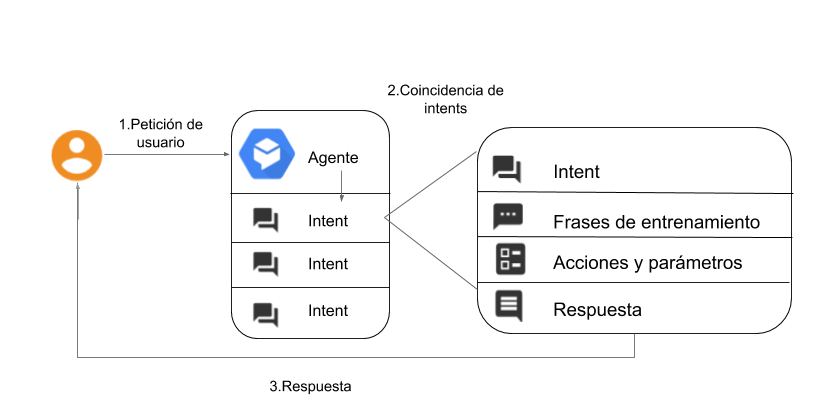
\includegraphics[width = 0.80\textwidth]{Figuras/FlujoCoincidencias.png}
         \end{center}
         \caption{\label{fig:FlujoCoincidencias}Flujo para identificar coincidencias y responder al usuario. Fuente: Google Cloud.}
     \end{figure}
     
     \newpage
     
     \item \textbf{Entidades}. Una entidad es una propiedad que Dialogflow utiliza para responder a una petición del usuario. Normalmente se trata de una palabra clave que contiene la petición como un nombre, fecha, localización, número, etc. Cuando el usuario realiza la petición, Dialogflow busca las entidades y extrae sus valores en forma de parámetros.
     
     Existe un conjunto predefinido de entidades del sistema para detectar coincidencias con muchos tipos comunes de datos. Si estas entidades no son suficientes, se pueden definir todas las entidades que se deseen para detectar coincidencias con datos personalizados. Por ejemplo, se puede definir la entidad PedidoID, como puede observarse en la siguiente figura:
     
     \begin{figure}[ht]
         \begin{center}
            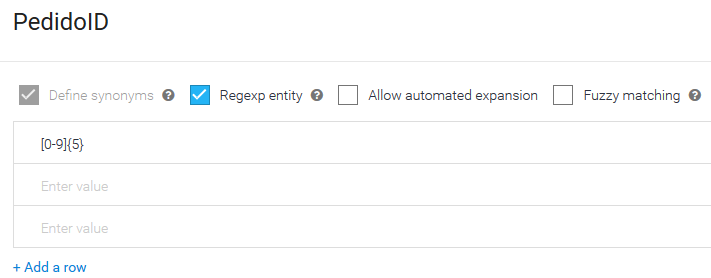
\includegraphics[width = 0.95\textwidth]{Figuras/Entidades.PNG}
         \end{center}
         \caption{\label{fig:DialogflowEntities}DialogFlow. Entidades}
     \end{figure}
     
     En la figura puede apreciarse que se ha definido una expresión regular para identificar los números de pedido.
     
     \newpage
     
     \item \textbf{Contextos}. Este concepto es semejante al usado en el lenguaje natural. Si una persona dice "es rojo", se necesita conocer el contexto para saber a qué se está refiriendo. De forma análoga, Dialogflow necesita un contexto para identificar el intent que se corresponde con la petición del usuario.
     
     Es un concepto importante, puesto que, permite tomar decisiones basadas en las respuestas anteriores, arreglar conversaciones que puede que se hayan roto por cualquier motivo y también ramificar la conversación en diferentes intents para crear una conversación fluida con el usuario.
     
     \item \textbf{Eventos}. Sirven para activar un intent sin que el usuario haga ninguna consulta. Por ejemplo, cuando el usuario abre el chat para comenzar una conversación con el bot se invoca al evento de bienvenida genérico "Welcome".
     
     \item \textbf{Fulfillments y Webhooks}. Permiten la comunicación del agente con otros servicios externos. Por defecto, el agente ofrece al usuario una respuesta predefinida en función del intent con el que se haya encontrado una coincidencia, sin embargo mediante los fulfillments el agente envía una solicitud al servicio webhook que tiene información sobre dicho intent. Un webhook no es más que un destino final en un servidor con el que se prevé contactar. De esta forma, el sistema realiza una acción determinada ante la petición efectuada por el agente y le responde con información sobre como proceder.
     
     Por ejemplo: si un usuario quiere reservar una habitación de hotel para Semana Santa, el servicio puede comprobar la base de datos y comunicarle al usuario si hay alguna habitación disponible en esas fechas.
     
     Para crear un webhook solo es necesario indicar la URL del destino final donde se van recoger las peticiones. Cada webook está asignado a un intent de modo que cuando se produce una coincidencia entre la entrada del usuario y dicho intent, se realizará una petición al servicio que incluirá en forma de JSON la información que el agente ha extraído del intent. 
     
     \begin{figure}[ht]
         \begin{center}
            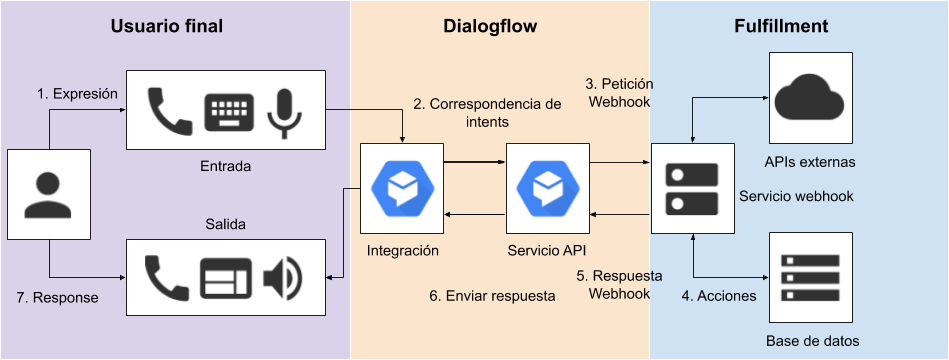
\includegraphics[width = 0.95\textwidth]{Figuras/Diagrama fulfillment.png}
         \end{center}
         \caption{\label{fig:DialogflowFulfillments}Flujo de fulfillment. Google Cloud.}
     \end{figure}
     
\end{itemize}